\documentclass[11pt]{article}

\usepackage[margin=1in]{geometry}
\usepackage[T1]{fontenc}
\usepackage[utf8]{inputenc}
\usepackage{lmodern}
\usepackage{microtype}
\usepackage{caption}
\captionsetup[figure]{
  labelformat=empty,
  justification=centering,
  font=small
}
\usepackage{amsmath, amssymb, mathtools}
\usepackage{booktabs}
\usepackage{array}
\usepackage{enumitem}
\usepackage{graphicx}
\usepackage{xcolor}
\usepackage{hyperref}
\usepackage[nameinlink,noabbrev]{cleveref}

\usepackage{tikz}
\usepackage{pgfplots}
\pgfplotsset{compat=1.18}
\usetikzlibrary{arrows.meta, positioning, shapes.geometric, shapes.misc, fit, calc}

\definecolor{btc}{RGB}{247,147,26}
\definecolor{lightgraybox}{RGB}{248,248,248}
\definecolor{midgray}{RGB}{95,95,95}

\hypersetup{
  colorlinks=true,
  linkcolor=black,
  citecolor=black,
  urlcolor=btc
}

\setlength{\parindent}{1.5em}
\setlength{\parskip}{0pt}

\newcommand{\event}{\texttt{event}}
\newcommand{\receipt}{\texttt{receipt}}
\newcommand{\subject}{\texttt{subject}}
\newcommand{\signedamount}{\texttt{signed\_amount}}
\newcommand{\pubkey}{\texttt{pubkey}}
\newcommand{\timestampfield}{\texttt{timestamp}}
\newcommand{\sigfield}{\texttt{sig}}
\newcommand{\eventid}{\texttt{event\_id}}
\newcommand{\acceptedts}{\texttt{accepted\_timestamp}}
\newcommand{\nodesig}{\texttt{node\_sig}}

\title{\textbf{Chronicle: Bringing Trust and Accountability\\to the Web}}
\author{Luka Dover \\
\small \url{https://chronicle-network.org}}
\date{}

\begin{document}

\maketitle

\begin{abstract}
The internet lacks a general public signal of trust. Existing signals such as likes, reviews, follows, and platform-local reputation are useful, but they are cheap to produce, easy to manipulate, fragmented across platforms, and often centrally controlled. We propose a protocol for costly public orientation on the web. Participants publish signed orientations toward or away from arbitrary subjects, expressed through publicly verifiable sacrifice. Nodes accept these events, relay them in real time, group them into batches, compute a Merkle root for each batch, and anchor that root to Bitcoin. After anchoring, nodes publish the full batch data off chain, allowing anyone to verify the anchor and reconstruct the public record. From this published data, downstream services can compute actor reputation and subject trust profiles using signed PageRank-style methods. Nodes do not need global coordination, and they do not need to provide full query interfaces. Their role is simply to accept valid events, anchor batch roots, and publish the corresponding batch data. We present the protocol structure and outline a reference signed PageRank algorithm for computing reputation and trust from the resulting public record.

\end{abstract}

\section{Introduction}

Interactions on the internet constantly depend on trust judgments. A user deciding whether to click a link, open an email, rely on a seller, follow an account, or use a service is always making some estimate of likely outcomes. Existing trust mechanisms such as reviews, ratings, follows, and platform-local reputation work well enough in many cases, but they remain cheap to produce, easy to manipulate, fragmented across platforms, and often centrally controlled. As a result, trust online remains local, weak, and easy to manipulate. A malicious website can appear legitimate, a spam sender can appear authentic, and a product can accumulate fake reviews that are difficult to distinguish from real ones. There is no widely adopted general-purpose internet protocol for signaling trust in a way that is portable, public, and accountable.

What is needed is a network for coordinating and aggregating distributed trust signals into a shared public map, allowing browsers, email clients, marketplaces, and social platforms to filter noise, surface substance, and respond more quickly to abuse. In this paper we propose a protocol that makes trust signaling costly, public, and portable. Instead of relying on cheap expression alone, it allows participants to publish signed orientation events toward or away from arbitrary subjects, backed by irreversible and provable sacrifice. Nodes accept these events, relay them, batch them, and anchor commitments to Bitcoin. From the resulting public graph, downstream services can compute actor reputation using a signed PageRank-style algorithm and derive subject trust profiles from reputation-weighted orientations. The effect is to make manipulation more expensive, trust more portable, and collective response easier, so that public trust maps can emerge from the costly orientations of many participants.

\section{Trust}

Trust can be understood as a summary of anticipated outcomes. A subject is trusted when interaction with it is expected to lead mostly to positive outcomes, distrusted when negative outcomes predominate, and controversial when expectations are split.

Let \(V\) denote anticipated outcome value associated with a subject. We define trust as
\[
\mathrm{Trust} = \Pr(V > 0) - \Pr(V < 0) \in [-1,1],
\]
so that trust measures the balance of positive and negative anticipated outcomes.

A trust profile visualizes that distribution. In the simplified figure below, \(-1\) and \(+1\) denote negative and positive outcomes respectively.

\begin{figure}[htbp]
\centering
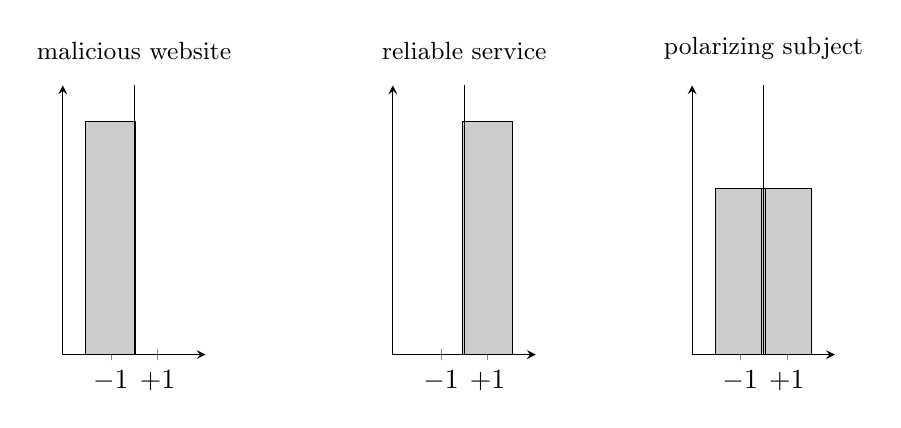
\begin{tikzpicture}
\begin{axis}[
    width=0.28\textwidth,
    height=5.0cm,
    ybar,
    bar width=18pt,
    ymin=0, ymax=6,
    xmin=-1.8, xmax=1.8,
    xtick={-1,1},
    xticklabels={$-1$,$+1$},
    ytick=\empty,
    axis lines=left,
    axis y line*=left,
    axis x line=bottom,
    title={malicious website},
    title style={font=\small},
    enlarge x limits=0.35
]
\addplot[draw=black, fill=black!20] coordinates {(-1,5.2) (1,0.0)};
\draw[thin] (axis cs:0,0) -- (axis cs:0,6);
\end{axis}

\begin{axis}[
    at={(5.1cm,0)},
    anchor=origin,
    width=0.28\textwidth,
    height=5.0cm,
    ybar,
    bar width=18pt,
    ymin=0, ymax=6,
    xmin=-1.8, xmax=1.8,
    xtick={-1,1},
    xticklabels={$-1$,$+1$},
    ytick=\empty,
    axis lines=left,
    axis y line*=left,
    axis x line=bottom,
    title={reliable service},
    title style={font=\small},
    enlarge x limits=0.35
]
\addplot[draw=black, fill=black!20] coordinates {(-1,0.0) (1,5.2)};
\draw[thin] (axis cs:0,0) -- (axis cs:0,6);
\end{axis}

\begin{axis}[
    at={(8.9cm,0)},
    anchor=origin,
    width=0.28\textwidth,
    height=5.0cm,
    ybar,
    bar width=18pt,
    ymin=0, ymax=6,
    xmin=-1.8, xmax=1.8,
    xtick={-1,1},
    xticklabels={$-1$,$+1$},
    ytick=\empty,
    axis lines=left,
    axis y line*=left,
    axis x line=bottom,
    title={polarizing subject},
    title style={font=\small},
    enlarge x limits=0.35
]
\addplot[draw=black, fill=black!20] coordinates {(-1,3.7) (1,3.7)};
\draw[thin] (axis cs:0,0) -- (axis cs:0,6);
\end{axis}
\end{tikzpicture}
\end{figure}

If the internet is to produce a public trust signal, it must produce credible evidence about that distribution. Existing systems do provide reviews, ratings, and warnings, but because those signals are cheap to produce and easy to manipulate, they cannot by themselves generate a reliable public map.

\section{Costly Orientation Events}

The solution starts with the concept of a costly orientation event: a signed signal toward or away from a subject that is expressed through irreversible sacrifice. The sign expresses direction and the amount expresses magnitude. The sacrifice is not a payment to another party, but a provable destruction of value. That distinction matters: payments can be routed, refunded, or cycled among cooperating actors, whereas destruction makes commitment publicly legible and difficult to game.

\[
\texttt{event} =
[\texttt{kind},\ \texttt{subject},\ \texttt{amount},\ \texttt{pubkey},\ \texttt{created\_at},\ \texttt{sig}]
\]

A positive amount orients toward the subject. A negative amount orients away from it. The signature proves that the event was created by the holder of the corresponding public key.

For example:

\[
\texttt{["web:domain", "scam.shop", -100, user\_pubkey, created\_at, sig]}
\]
\[
\texttt{["web:domain", "example.com", +50, user\_pubkey, created\_at, sig]}
\]

A subject may be any protocol-defined identifier or entity. Subjects can include domains, URLs, pubkeys, nodes, user accounts, or prior orientation events. This allows the same primitive to represent first-order trust judgments, direct judgments about actors or infrastructure, and later acknowledgment of whether a prior orientation proved useful. Because subjects may include actors and prior events, the public record forms an explicit orientation graph rather than a flat list of ratings.

\section{Nodes}

Costly orientation events need an execution layer, which is provided by public nodes. A node is a paid public service that accepts valid signed events from clients, charges a fee for processing them, groups accepted events into a batch, computes a cryptographic root for that batch, and anchors that root to Bitcoin \cite{nakamoto2008bitcoin}. The anchor transaction must destroy at least as much bitcoin as the total sacrifice represented by the events in the batch. This allows many orientation events to share a single public anchor while preserving independent verifiability.

For each batch, the node orders accepted events deterministically, hashes them into a Merkle tree \cite{merkle1987digital}, binds the resulting root to its own public key, and places that commitment in an \texttt{OP\_RETURN} output of a Bitcoin transaction.

\begin{figure}[htbp]
\centering
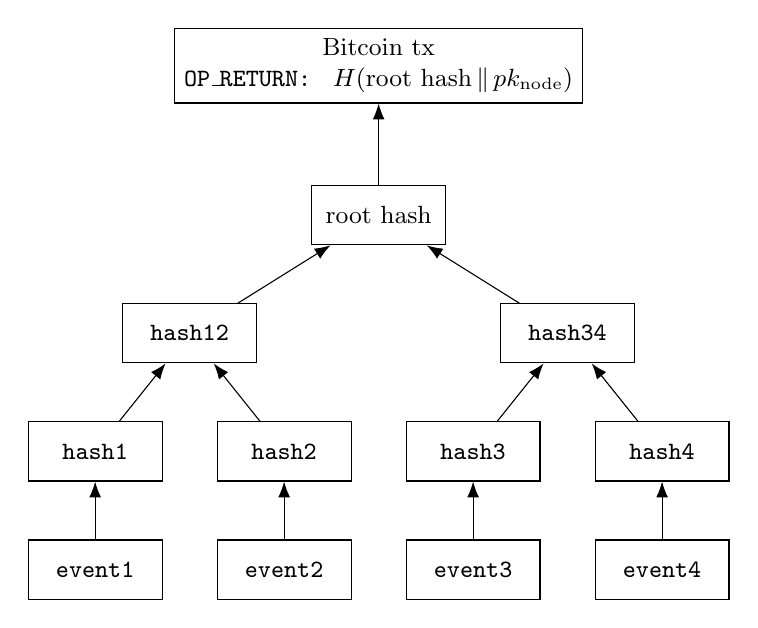
\begin{tikzpicture}[
    font=\small,
    box/.style={draw, rectangle, minimum height=0.75cm, minimum width=1.7cm, align=center},
    widebox/.style={draw, rectangle, minimum height=0.95cm, minimum width=4.2cm, align=center},
    arrow/.style={-{Latex[length=2mm]}, thin}
]

% Events
\node[box] (e1) at (0,0) {\texttt{event1}};
\node[box] (e2) at (2.4,0) {\texttt{event2}};
\node[box] (e3) at (4.8,0) {\texttt{event3}};
\node[box] (e4) at (7.2,0) {\texttt{event4}};

% Leaf hashes
\node[box] (h1) at (0,1.5) {\texttt{hash1}};
\node[box] (h2) at (2.4,1.5) {\texttt{hash2}};
\node[box] (h3) at (4.8,1.5) {\texttt{hash3}};
\node[box] (h4) at (7.2,1.5) {\texttt{hash4}};

\draw[arrow] (e1) -- (h1);
\draw[arrow] (e2) -- (h2);
\draw[arrow] (e3) -- (h3);
\draw[arrow] (e4) -- (h4);

% Internal hashes
\node[box] (h12) at (1.2,3.0) {\texttt{hash12}};
\node[box] (h34) at (6.0,3.0) {\texttt{hash34}};

\draw[arrow] (h1) -- (h12);
\draw[arrow] (h2) -- (h12);
\draw[arrow] (h3) -- (h34);
\draw[arrow] (h4) -- (h34);

% Root
\node[box] (root) at (3.6,4.5) {root hash};

\draw[arrow] (h12) -- (root);
\draw[arrow] (h34) -- (root);

% Bitcoin transaction / OP_RETURN
\node[widebox] (tx) at (3.6,6.4)
{Bitcoin tx \\ \texttt{OP\_RETURN: } $H(\text{root hash} \,\|\, pk_{\mathrm{node}})$};

\draw[arrow] (root) -- (tx);

\end{tikzpicture}
\caption{Events are grouped into a batch, hashed into a Merkle root, and anchored to Bitcoin.}
\end{figure}

After anchoring, the node publishes the full batch data off chain. Anyone can then recompute the batch root from the published events and verify that the corresponding Bitcoin transaction contains the correct commitment and sufficient sacrifice. Published batches therefore form a node’s public operational history, which anyone can inspect to evaluate performance and reliability.

\section{Real-Time Coordination}

Bitcoin anchoring provides public finality, but many coordination problems require a faster response than block times allow. A scam link, malicious sender, or compromised account may need to be signaled immediately, not only after the next anchor is published. To support real-time coordination, nodes relay accepted events as soon as they are received.

When a node accepts an orientation event, it immediately broadcasts the event together with a receipt. The event shows that the actor signed the orientation. The receipt shows that the node accepted responsibility for including the event in a later anchored batch. This allows clients and downstream services to respond before final anchoring on Bitcoin.

Receipts make node responsibility public. If a node repeatedly emits receipts that are not later honored in published batches, that failure becomes visible in the public record. The node can then itself become the subject of negative orientation within the same protocol, damaging its standing and reducing future trust in its service.

\section{Incentives}

The protocol relies on incentives at three levels: the incentives of nodes that execute and publish events, the incentives of participants whose orientations shape the trust map, and the incentives of downstream service providers that store, index, audit, and serve useful views of the public data.

Nodes are paid public services. They charge fees for accepting events, relaying them, anchoring them, and publishing verifiable batch data. This gives nodes a direct incentive to remain available, honor receipts, and maintain a public record of reliable work. A node that censors events, fails to publish its batches, or repeatedly emits receipts that are not later honored, damages its own standing and risks losing future traffic to competing nodes.

Participants are incentivized not only by direct influence over trust profiles, but also by reputation. An orientation that later proves useful for others can itself become the subject of later positive orientation. In this way, actors who repeatedly help others avoid harm or find value can accumulate public reputation and with it greater influence over future trust-map computation.

Nodes are execution and publication services, not query engines. Downstream service providers can build on top of the published data to provide storage, indexing, trust-map APIs, reputation computation, and node auditing. These services can also be monetized. Providers that make the public data easier to access, interpret, and use have a direct economic incentive to improve the quality of the ecosystem while helping keep nodes accountable. As more services mirror and process published batches, storage becomes more redundant and the public record more resilient.

The incentives of the system are therefore recursive. Nodes are rewarded for operational honesty and reliability. Participants are rewarded for producing orientations that others later find useful. Downstream service providers are rewarded for making the public trust record usable. Manipulation is not eliminated, but it becomes more expensive, more public, and more accountable.

\section{Computing Trust}

Services that compute trust lie outside the strict protocol boundary. The protocol publishes a public graph of costly orientations; downstream services interpret that graph and derive useful signals from it. Different services may use different algorithms, and those algorithms will evolve over time. Their design nonetheless matters, because it shapes how influence accumulates and how the public record is interpreted.

Published orientation data is useful even in the simplest case. A first estimate of trust can be obtained by aggregating net signed sacrifice toward a subject. If many participants independently orient away from a domain, the resulting trust profile shifts negative. If many orient toward it, the profile shifts positive. Even this simple approach already produces a stronger public signal than systems based on costless ratings or reviews.

A better algorithm, however, should not treat every source equally. Some actors prove more useful than others. An orientation made by an actor whose prior signals repeatedly helped others avoid harm or find value should count more than an orientation made by an unknown or consistently misleading actor. Raw trust profiles should therefore be weighted by reputation.

\begin{figure}[htbp]
\centering
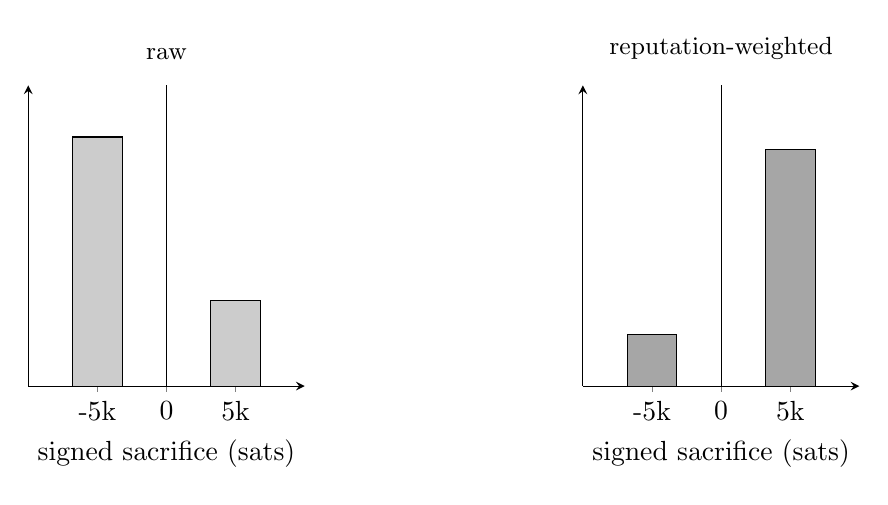
\begin{tikzpicture}
\begin{axis}[
    width=0.42\textwidth,
    height=5.4cm,
    ybar,
    bar width=18pt,
    ymin=0, ymax=7,
    xmin=-10000, xmax=10000,
    xtick={-5000,0,5000},
    xticklabels={-5k,0,5k},
    scaled x ticks=false,
    ytick=\empty,
    axis lines=left,
    axis y line*=left,
    axis x line=bottom,
    xlabel={signed sacrifice (sats)},
    title={raw},
    title style={font=\small},
    enlarge x limits=false
]
\addplot[draw=black, fill=black!20] coordinates {
(-5000,5.8) (5000,2.0)
};
\draw[thin] (axis cs:0,0) -- (axis cs:0,7);
\end{axis}

\begin{axis}[
    at={(8.8cm,0)},
    anchor=origin,
    width=0.42\textwidth,
    height=5.4cm,
    ybar,
    bar width=18pt,
    ymin=0, ymax=7,
    xmin=-10000, xmax=10000,
    xtick={-5000,0,5000},
    xticklabels={-5k,0,5k},
    scaled x ticks=false,
    ytick=\empty,
    axis lines=left,
    axis y line*=left,
    axis x line=bottom,
    xlabel={signed sacrifice (sats)},
    title={reputation-weighted},
    title style={font=\small},
    enlarge x limits=false
]
\addplot[draw=black, fill=black!35] coordinates {
(-5000,1.2) (5000,5.5)
};
\draw[thin] (axis cs:0,0) -- (axis cs:0,7);
\end{axis}
\end{tikzpicture}
\caption{The same raw sacrifice can imply a different trust profile once source reputation is taken into account.}
\end{figure}

This makes trust computation recursive. A subject's score depends on the costly orientations pointed toward it, weighted by the reputations of the actors who made them. An actor's reputation depends on the public graph of orientations toward that actor and toward the actor's prior events. A useful warning can therefore strengthen the reputation of the actor who made it, while a misleading endorsement can weaken it.

The reference algorithm in the appendix adapts PageRank \cite{page1999pagerank} to this signed orientation graph. In PageRank, links route importance between pages. In the reference algorithm, costly orientations route influence between actors. Positive inbound sacrifice supplies the external rank source, signed actor orientations form the influence matrix, and subject scores are computed afterward from reputation-weighted orientations.

The distinction is important. Subjects such as domains, URLs, email addresses, and phone numbers receive trust scores, but they do not recursively distribute influence. Actors do. In this sense, Chronicle creates an explicit public graph in which participants continuously determine how influence should be distributed over trust maps of subjects.

This differs from the web graph PageRank originally analyzed. A hyperlink was an ambiguous and indirect signal: it could mean endorsement, citation, criticism, convenience, or spam. Because PageRank inferred orientation from this proxy, the ranking signal degraded once the proxy became profitable to manipulate, a familiar case of Goodhart's Law \cite{goodhart1975problems}. A Chronicle event is explicit, signed, directional, and costly. It says who oriented, what they oriented toward, in which direction, and with what magnitude.

The aim is therefore similar to PageRank, but applied to a different signal substrate. PageRank extracted importance from a graph of hyperlinks. The reference algorithm extracts actor reputation from a graph of public costly orientation, then uses that reputation to weight subject trust scores.

\section{Resistance to Manipulation}

A public trust map becomes harder to bend as costly history accumulates. An actor can always spend money and publish new orientations, but influence should not come cheaply. Reputation must be earned through a visible record of orientations that others later find useful. That takes time, repeated sacrifice, and later acknowledgment from participants who benefited from those signals. Once earned, reputation gives an actor greater weight in future trust computation. But using that influence to push harmful or misleading orientations should place the same reputation at risk.

The protocol provides the public graph of orientations, but trust-computation algorithms determine how that graph is interpreted. Those algorithms therefore shape behavior: they influence which actions build credibility, how quickly new sacrifice can move the map, and how easily accumulated influence can be abused. To resist manipulation, robust algorithms should account for three structural properties.

\paragraph{Capital inertia.}
A graph with a large body of anchored sacrifice should be hard to move. In a mature graph with millions of participants and a large accumulated history of sacrifice, a new manipulator should need substantial sacrifice before the map shifts meaningfully.

\paragraph{Historical advantage.}
A long public history of sacrifice should count more than an equal amount that appears suddenly. Time matters because a long public record has had more opportunity to be exposed to correction, contradiction, and acknowledgment.

\paragraph{Reputational fragility.}
Reputation should be slow to earn and easier to lose. An actor may gain influence through a sustained public record of useful orientations, yet lose that influence quickly once later evidence reveals a pattern of harmful or misleading behavior.

These are not properties of the protocol, but of the algorithms built on top of it. The protocol makes these properties computationally available by publishing a public graph of signed, costly, time-ordered orientations that can target subjects, actors, and prior events.

\section{Conclusion}

We have proposed a base-layer protocol for public trust signaling on the internet. Instead of relying on cheap, fragmented, and platform-local signals, the protocol makes orientation costly and publicly verifiable. Nodes operate without global coordination. They accept fee-paying events, relay them, group them into batches, anchor batch roots to Bitcoin, and publish the corresponding batch data off chain. Downstream services can then use that public record to estimate trust profiles, compute reputation, and build useful interfaces on top.

We have also outlined a reference signed PageRank algorithm in which actor reputation is computed recursively from the public orientation graph, and subject trust scores are computed from reputation-weighted orientations. In this way, the same orientation graph that records costly action can also support recursive reputation and increasing resistance to manipulation over time.

The protocol is not a replacement for reviews, ratings, or existing reputation systems. Reviews provide context and explanation; Chronicle adds magnitude and accountability through publicly verifiable sacrifice. 

The protocol changes the economics of influence by making trust signaling costly and accountable. It offers a shared coordination layer through which trust-relevant judgments can become more public, more reusable across contexts, and more resistant to manipulation across the web.

\appendix

\section{Reference Signed PageRank Algorithm}

This appendix describes one PageRank-style reference algorithm for computing actor reputation and subject quality from a Chronicle graph. The purpose is to outline a basic way the orientation graph can be interpreted. It omits several features that production trust-computation methods may need, such as time decay, and a stronger treatment of adversarial clusters. Many other ranking methods can be developed on top of the same public record.

\subsection{From PageRank to Signed Reputation}

PageRank computes recursive importance from a graph of links between pages \cite{page1999pagerank}. If \(A\) is the link matrix and \(R\) is the rank vector, PageRank seeks a fixed point of the form \(R = cRA\). Operationally, this fixed point is computed by repeatedly propagating rank through the graph until the rank vector stabilizes.

With an external rank source \(E\), the damped iterative form can be written as

\[
R^{(t+1)} = dR^{(t)}A + (1-d)E,
\]

where \(d \in (0,1)\) is the damping factor. The source \(E\) injects rank from outside the link graph and prevents rank from being trapped in sinks.

Our algorithm keeps this fixed-point structure but changes the meaning of the graph.

\begin{table}[h]
\centering
\begin{tabular}{ll}
\hline
\textbf{PageRank} & \textbf{Reference algorithm} \\
\hline
page & actor \\
hyperlink & signed costly orientation \\
page rank & actor reputation \\
external rank source \(E\) & positive inbound sacrifice \\
link matrix \(A\) & signed influence matrix \\
\hline
\end{tabular}
\end{table}

The result is a signed PageRank-style computation over actors.

\subsection{Influence Matrix}

Let \(o_{u,v}\) be the signed total orientation from actor \(u\) toward actor \(v\), including orientations toward \(v\) directly and orientations toward events authored by \(v\). For each actor \(u\), define total outgoing sacrifice as \(S_u = \sum_{x \ne u} |o_{u,x}|\). Self-loops are not routed through the recursive influence matrix.

The signed influence matrix is defined by \(A_{u,v} = o_{u,v}/S_u\) when \(S_u > 0\) and \(u \ne v\), and by \(A_{u,v}=0\) otherwise. Thus the absolute values in each non-empty row sum to one: \(\sum_v |A_{u,v}| = 1\).

Actors with no outgoing orientations have zero rows. Unlike ordinary PageRank treatments that redistribute dangling-page rank across the graph, this algorithm does not treat a silent actor as implicitly orienting toward everyone.

The matrix \(A\) routes existing reputation. The source vector \(E\) determines where reputation enters.

\subsection{External Rank Source}

The external rank source \(E\) is derived from positive inbound sacrifice. Let \(b_v\) be the total positive sacrifice oriented toward actor \(v\), including positive orientations toward \(v\) directly and positive orientations toward events authored by \(v\).

Only positive orientations contribute to \(E\). Negative orientations may affect reputation through signed recursive propagation, but they do not create positive source rank.

This algorithm does not attempt to distinguish self-funded and other-funded source rank. Actors can create multiple keys, so that distinction is not reliable at the graph level. What matters for the reference computation is that the sacrifice is public, costly, and irreversible.

Let \(B = \sum_x b_x\). If \(B > 0\), set \(E_v = b_v/B\). If \(B = 0\), use the uniform source \(E_v = 1/n\). In either case, \(E\) is a nonnegative source vector normalized so that \(\|E\|_1 = 1\).

\subsection{Iteration}

Actor reputation is initialized from the source, \(R^{(0)} = E\), and then iterated until convergence:

\[
R^{(t+1)} = dR^{(t)}A + (1-d)E.
\]

In the reference implementation, \(d = 0.85\). Iteration stops when \(\|R^{(t+1)} - R^{(t)}\|_1 < \varepsilon\).

Unlike ordinary PageRank, the reputation vector is signed. It is not interpreted as a probability distribution and is not required to satisfy \(\|R\|_1 = 1\). For output, the raw vector may be rescaled so displayed actor reputation lies in the range \([-1,1]\).

\subsection{Subject Quality}

After actor reputation converges, subjects are scored directly. The subject quality score \(Q(s)\) is the reputation-weighted sum of orientations toward subject \(s\), using only actors with positive reputation:

\[
Q(s)
=
\sum_{e:\,\mathrm{subject}(e)=s}
\mathrm{amount}(e)\cdot
\max\!\bigl(0,R_{\mathrm{actor}(e)}\bigr).
\]

Actors with negative reputation contribute no weight. This avoids giving negatively reputable actors inverted authority. A large positive or negative orientation from an actor with negative reputation does not move the subject score in this reference algorithm.

For output, subject scores may be rescaled so displayed values lie in the range \([-1,1]\).

\subsection{Event Contribution}

Event contribution explains which prior actions affected an actor's reputation. This is useful feedback for actors: reputation is not only a global score, but a trail of public orientations that helped or harmed it.

Events are not recursive reputation nodes in this reference algorithm. During reputation computation, an orientation toward a prior event is treated as an orientation toward the actor who authored that event. After reputation has converged, we can attribute part of the resulting reputation flow back to the specific events that were judged. This makes it possible to show which public actions affected an actor's reputation without making every event a full recursive node in the matrix.

The method is simple: look at later orientations toward a prior event and weight each one by the final reputation of the actor who made it. Let \(\mathcal{H}(e)\) be the set of orientation events that target prior event \(e\). The contribution of \(e\) is

\[
C(e)
=
\sum_{h \in \mathcal{H}(e)}
\frac{d\,R_{\mathrm{actor}(h)}\,\mathrm{amount}(h)}
{S_{\mathrm{actor}(h)}}.
\]

Positive \(C(e)\) means the event helped its author's reputation; negative \(C(e)\) means it harmed it.

\subsection{Summary}

This reference algorithm adapts PageRank from a graph of hyperlinks into a signed influence matrix over public costly orientation.

The source vector \(E\) decides where reputation enters. The influence matrix \(A\) decides how reputation flows. The reputation vector \(R\) is the recursive actor score produced by repeated propagation. The subject quality score \(Q\) is computed afterward by weighting subject orientations according to actor reputation.

\begin{thebibliography}{9}

\bibitem{nakamoto2008bitcoin}
Satoshi Nakamoto.
\newblock \textit{Bitcoin: A Peer-to-Peer Electronic Cash System}.
\newblock 2008.
\newblock \url{https://bitcoin.org/bitcoin.pdf}

\bibitem{page1999pagerank}
Lawrence Page, Sergey Brin, Rajeev Motwani, and Terry Winograd.
\newblock \textit{The PageRank Citation Ranking: Bringing Order to the Web}.
\newblock Stanford InfoLab, Technical Report 1999-66, 1999.

\bibitem{merkle1987digital}
Ralph C. Merkle.
\newblock A Digital Signature Based on a Conventional Encryption Function.
\newblock In \textit{Advances in Cryptology --- CRYPTO '87}, Lecture Notes in Computer Science, Vol. 293.
\newblock Springer, 1988.

\bibitem{goodhart1975problems}
Charles A. E. Goodhart.
\newblock Problems of Monetary Management: The U.K. Experience.
\newblock In \textit{Papers in Monetary Economics}, Vol. 1.
\newblock Reserve Bank of Australia, 1975.

\end{thebibliography}
\end{document}